\chapter{Analysis and Specification of Requirements}

\section*{Introduction}

In this chapter, we will present the analysis and specification of Requirements. We start by presenting the specification of the requirements, illustrating them using the diagram of the global use cases. Then we will present our project architecture and our working environment, and finally we will present our product backlog and releases planning, and we will close our chapter with a conclusion.

\section{Requirements Specification}

In this section, we will define the actors of our application and the functional and non-functional Requirements that our application aims to fulfill.

\subsection{Identifying Actors}

We define actors as a shorthand for the roles played by entities outside the system that interact directly with them \cite{CockburnUML2002, CockburnWritingEffectiveUseCases2000}. In our system, we identify four types of actors:

\begin{itemize}
    \item \textbf{\textcolor{primary}{Super Admin}}: Responsible for the global configuration of the platform, they have extended privileges to manage administrators, oversee security, and ensure compliance. They can also configure advanced features and control all system resources.
    
    \item \textbf{\textcolor{primary}{Admin}}: In charge of the day-to-day management of the platform, they can add, modify, or delete listings, supervise agency and user profiles, and ensure smooth operations. They are also responsible for monitoring and assisting other actors.
    
    \item \textbf{\textcolor{primary}{Real Estate Agent}}: Dedicated to creating and updating real estate listings, they manage property information, handle investor requests, and finalize transactions related to sales or rentals. They can also coordinate property visits and propose tailored offers.
    
    \item \textbf{\textcolor{primary}{Investor}}: A user who wishes to browse and finance real estate projects. They have access to all available offers, can make investments in a few simple steps, and monitor the evolution of their portfolio. They also benefit from personalized insights to optimize their investments.
    
    \item \textbf{\textcolor{primary}{System}}: The entity that automatically manages all basic functionalities, such as authentication, notification generation, transaction validation, and adherence to security protocols. It ensures the coherence and reliability of the application at all times.
\end{itemize} 

\subsection{Functional Requirements}

\addtocontents{toc}{\protect\newpage}
After several meetings with our client, the various functional requirements of our application are illustrated as follows:

\subsubsection{For the Super Admin (Korpor)}
\begin{itemize}
    \item \textbf{Authenticate}: The super admin enters their credentials to access the advanced management console.
    \item \textbf{Log Out}: After viewing or updating global settings, they can securely log out.
    \item \textbf{Manage Admin Accounts}: Create, enable/disable, or modify admin profiles associated with different real estate companies.
    \item \textbf{Monitor Security \& Compliance}: Oversee transactions, data integrity, and regulatory adherence using specialized reporting and audit tools.
    \item \textbf{Configure Platform Features}: Define key parameters (payment methods, AI/blockchain integrations, etc.) and roll out feature updates.
    \item \textbf{View Global Reports}: Generate and analyze consolidated metrics (financials, user activity, transactions) for overall performance insights.
    \item \textbf{Moderate Content}: Review and remove any inappropriate or erroneous property listings or user-generated data.
\end{itemize} 

\subsubsection{For the Admin (Real Estate Company)}
\begin{itemize}
    \item \textbf{Authenticate}: The admin logs in with valid credentials to manage daily operations.
    \item \textbf{Log Out}: They can end their session to maintain account security.
    \item \textbf{Manage Real Estate Listings}: Add, update, or delete property listings visible to investors.
    \item \textbf{Oversee Real Estate Agents}: Create and manage agent accounts, assign properties, and monitor performance and commissions.
    \item \textbf{Track Transactions \& Commissions}: Review incoming payments, calculate commissions owed to agents, and track the history of completed deals.
    \item \textbf{Address Investor Inquiries}: Respond to questions or concerns from investors, ensuring a smooth user experience.
    \item \textbf{Access Agency Dashboard}: View comprehensive statistics on properties, sales, rentals, and market trends.
\end{itemize}

\subsubsection{For the Real Estate Agent}
\begin{itemize}
    \item \textbf{Authenticate}: The agent logs in to manage assigned properties and interact with potential investors.
    \item \textbf{Log Out}: Securely exit the account after completing tasks.
    \item \textbf{Manage Assigned Properties}: Create new listings, update property details, set prices, and upload images.
    \item \textbf{Handle Investment Requests}: Review purchase or rental offers, negotiate terms, and initiate contract finalization.
    \item \textbf{Contribute to AI Estimates}: Provide or refine data to improve AI-driven pricing and market analysis.
    \item \textbf{Maintain Client Relationships}: Communicate with investors, schedule property visits, and follow up on inquiries.
    \item \textbf{View Commissions}: Track earnings based on successful sales or rentals.
\end{itemize}

\subsubsection{For the Investor (Mobile App User)}
\begin{itemize}
    \item \textbf{Create an account \& authenticate}: Register to gain access to the platform's core features.
    \item \textbf{Log Out}: End the session to protect personal and financial data.
    \item \textbf{Browse Listings \& Invest}: Explore available properties, filter according to preferences, and commit to an investment in a few steps.
    \item \textbf{Track Portfolio}: Monitor owned assets, property status, and receive real-time updates on performance.
    \item \textbf{Make Payments}: Use integrated payment methods (credit cards, digital wallets, etc.) to complete transactions.
    \item \textbf{Access AI Recommendations}: View data-driven insights and return-on-investment estimates generated by the system.
    \item \textbf{Manage Withdrawals \& Earnings}: Withdraw profits, monitor rental income, or exit investments under the right conditions.
\end{itemize}

\subsubsection{For the System}
\begin{itemize}
    \item \textbf{Automate Authentication}: Validate credentials, manage sessions, and maintain user roles and permissions.
    \item \textbf{Generate Notifications}: Send real-time alerts (e.g., new listings, completed transactions, commission updates) to relevant users.
    \item \textbf{Ensure Compliance \& Security}: Leverage blockchain for data integrity, verify payments, and detect anomalies or fraudulent activities.
    \item \textbf{Coordinate AI Insights}: Aggregate and analyze real estate data to produce market predictions and price recommendations.
    \item \textbf{Maintain Transaction Consistency}: Update dashboards, user balances, and property statuses automatically upon each operation.
    \item \textbf{Optimize Performance}: Monitor server load, scale resources, and ensure a smooth, responsive application experience.
\end{itemize} 

\subsection{Non-functional Requirements}

In order to ensure the proper functioning of the decision-making system and to avoid any kind of anomaly, the implemented solution must meet a set of non-functional needs such as:

\begin{itemize}
    \item \textbf{Maintainability}: The system must be designed for simplicity so that tasks, updates, and bug fixes can be executed with minimal complexity \cite{DevOpsFoundation2023, FowlerRefactoring2018}.
    
    \item \textbf{Evolution}: Platform administration must remain attentive to user needs and feedback, continuously enhancing the services offered while preserving the application's utility and efficiency \cite{PoppendieckLean2012, KnibergLeanStartup2013}.
    
    \item \textbf{Security}: Robust security measures are essential. The platform must enforce strong authentication protocols, access privileges, and comprehensive data encryption (both at rest and in transit) \cite{ClerkAuthenticationDocs, OWASPSecurityPrinciples2021}. The integration of blockchain technology further ensures the immutability and integrity of sensitive information \cite{WangBlockchainRealEstate2023, McKinseyBlockchainRE2023}.
    
    \item \textbf{Efficiency}: The application must be effective in all circumstances, delivering prompt and reliable functionality regardless of external conditions \cite{KimDevOpsMethods2018, BassArchitecture2021}.
    
    \item \textbf{Performance}: The system must operate optimally across diverse environments. It should consistently provide a responsive and reliable experience, even under high transaction volumes or varying network conditions \cite{DockerArchitecture2023, ForsgreniDevOpsMetrics2023}.
\end{itemize} 

\section{Requirements Analysis}

In this section, we'll outline the various features that our app should offer, using a general use case diagram \cite{CockburnUML2002}.

\subsection{General use case diagram}

Below, we present the various actors of the application and the actions they are authorized to perform.
The overall diagram is illustrated in Figure \ref{fig:use-case-diagram}:

\begin{figure}[htbp]
    \centering
    % Replace with actual image file once available
    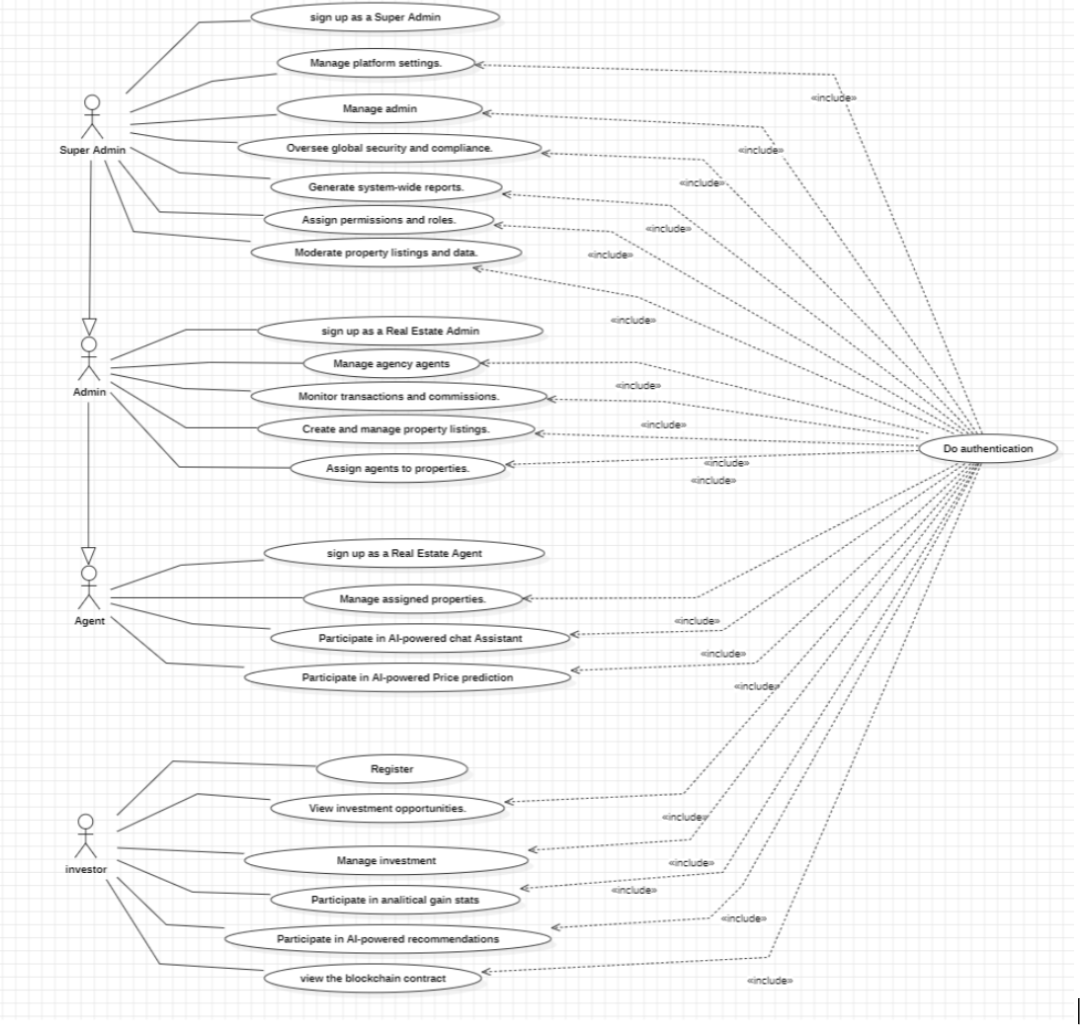
\includegraphics[width=0.6\textwidth]{images/diagram de case d utilisation general.png}
    \caption{General use case diagram}
    \label{fig:use-case-diagram}
\end{figure}
\newpage
\section{Software architecture}

Before starting the design and development of any computerized system, it is essential to prepare the architecture.

\subsection{Physical architecture}

 The physical architecture of Korpor leverages modern, scalable technologies to deliver a seamless investment platform. The frontend is built with Expo, React, and TypeScript using Vite \cite{ViteJSWebsite} for rapid development and Tanstack for robust state management and data visualization, while Storybook supports isolated UI component development \cite{StorybookDocs2022}. The backend relies on Express.js \cite{ExpressJSWebsite} with user authentication managed by Clerk \cite{ClerkAuthenticationDocs}, containerization via Docker \cite{DockerArchitecture2023}, and MySQL \cite{MySQLWebsite} for data storage hosted on Microsoft Azure \cite{AzureCloudServices2024}. Integrated AI modules provide personalized insights \cite{JohnsonAIPropertyValuation2024}, and blockchain technology ensures transactional security and data immutability \cite{WangBlockchainRealEstate2023, McKinseyBlockchainRE2023}. This setup is further supported by GitHub \cite{GithubWebsite} for version control, Postman \cite{PostmanWebsite} for API testing, and end-to-end testing tools like Maestro and Playwright \cite{PlaywrightDocs2023}, with architectural designs and documentation maintained using StarUML \cite{StarUMLWebsite} and Overleaf.

\begin{figure}[htbp]
    \centering
    % Replace with actual image file once available
    % \includegraphics[width=0.85\textwidth]{images/physical_architecture.png}
    \caption{Deployment diagram}
    \label{fig:physical-architecture}
\end{figure}

\subsection{Logical architecture}

To better manage code organization and ensure maintainability, we've designed our application based on the MVC (Model-View-Controller) \cite{SunardiMVC2019, GammaPatterns1994} architectural pattern:

\begin{itemize}
    \item \textbf{Model}: Represents application data and business logic.
    \item \textbf{View}: Presents data to users through interfaces.
    \item \textbf{Controller}: Processes incoming requests, performs operations using Models, and returns appropriate Views.
\end{itemize}

Architecture Components:
\begin{itemize}
    \item \textbf{Model:} The MySQL database serves as the core data source, responsible for storing and managing application data, including user profiles, real estate listings, transactions, and investment records. The data layer interacts with the backend through ORM or query-based operations, ensuring efficient data retrieval and persistence.
    
    \item \textbf{Controller:} The Express.js backend acts as the intermediary between the database and the frontend, handling user requests, business logic, and data validation. It processes API calls from the frontend and interacts with services such as Clerk for authentication, AI modules for predictive analytics, and blockchain integration for secure transactions.
    
    \item \textbf{View:} The frontend is built with React, TypeScript, and TanStack tools, ensuring a responsive and interactive UI. The frontend communicates with the backend via API requests, displaying dynamic content and allowing seamless user interaction.
\end{itemize}

The logical architecture is illustrated in Figure \ref{fig:logical-architecture}.

\begin{figure}[htbp]
    \centering
    % Replace with actual image file once available
    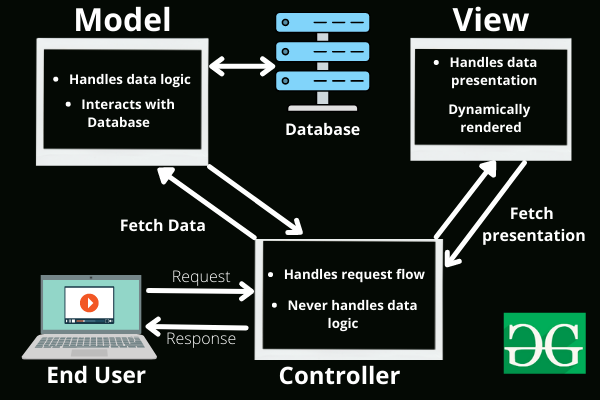
\includegraphics[width=0.9\textwidth]{images/logique.png}
    \caption{Logical architecture}
    \label{fig:logical-architecture}
\end{figure}

Request Flow:
\begin{enumerate}
    \item A user action (e.g., viewing property listings) triggers a request in the frontend.
    \item The request is sent to the backend via an API call.
    \item The Express.js controller processes the request, interacting with the database and other services.
    \item Data is retrieved, processed, and returned as a response.
    \item The frontend updates the UI dynamically based on the received data.
\end{enumerate}

This structured approach ensures a scalable, secure, and high-performance system, optimizing Korpor's real estate investment and management operations \cite{KimDevOpsMethods2018}.

\section{Work Environment}

In this part, we will talk about our work environment, focusing on different aspects:
our material environment, the techniques we used in the realization of our project as well as the tools we used in our report, the product backlog and sprint planning, and finally, we will conclude this section \cite{BeckXP2004, MartinCleanArchitecture2017}.

\subsection{Physical environment}

The work was carried out by a laptop computer that is equipped with these detailed features presented in Table \ref{tab:physical-env} below:

\begin{table}[htbp]
    \centering
    \begin{tabular}{|l|l|}
        \hline
        \textbf{Computer Name} & MSI \\
        \hline
        \textbf{Processor} & i5 10th gen \\
        \hline
        \textbf{Hard disk} & 512 Go SSD \\
        \hline
        \textbf{RAM} & 24.0 Go \\
        \hline
        \textbf{Operating system} & Windows 11 Pro \\
        \hline
    \end{tabular}
    \caption{Physical environment}
    \label{tab:physical-env}
\end{table}

\subsection{Used technologies}

% Define a command for technology icons to make it easier to adjust if needed
\newcommand{\techicon}[1]{%
  \includegraphics[height=1em]{images/icons/#1.png}%
}

\subsubsection*{\protect\techicon{expo} Expo}

Expo is an open-source platform for making universal native apps for Android, iOS, and the web with JavaScript and React.

\subsubsection*{\protect\techicon{typescript} TypeScript}
                                                                
TypeScript (abbreviated as TS) is a free and open-source high-level programming language developed by Microsoft that adds static typing with optional type annotations to JavaScript \cite{TypeScriptDocs2023}. It is designed for the development of large applications and transpiles to JavaScript.

\subsubsection*{\protect\techicon{tanstack} Tanstack}
                                                                      
High-quality open-source software for web developers \cite{TanstackWebsite}. Headless, type-safe, \& powerful utilities for Web Applications, Routing, State Management, Data Visualization, Datagrids/Tables, and more.

\subsubsection*{\protect\techicon{clerk} Clerk}
                                                                        
Clerk \cite{ClerkAuthenticationDocs} is a complete suite of embeddable UIs, flexible APIs, and admin dashboards to authenticate and manage your users.

\subsubsection*{\protect\techicon{maestro} Maestro}
                                                                        
Maestro \cite{MaestroDocs2022} is the simplest, most powerful, and most trusted end-to-end testing platform for mobile and web apps.

\subsubsection*{\protect\techicon{azure} Google cloud platform}

Google cloud platform, or just GCP, is the cloud computing platform developed by Google. It has management, access and development of applications and services to individuals, companies, and governments through its global infrastructure.

\subsubsection*{\protect\techicon{github} GitHub}

GitHub \cite{GithubWebsite} is a cloud-based service that helps developers store and manage their code, as well as track and control changes to their code.

\subsubsection*{\protect\techicon{express} Express.js}

Express.js \cite{ExpressJSWebsite} is a minimal and flexible Node.js \cite{NodeJSWebsite} web application framework that provides a list of features for building web and mobile applications easily.

\subsubsection*{\protect\techicon{postman} Postman}

Postman \cite{PostmanWebsite} is an API platform for building and using APIs. Postman simplifies each step of the API lifecycle and streamlines collaboration so you can create better APIs—faster.

\subsubsection*{\protect\techicon{vite} Vite}

Vite \cite{ViteJSWebsite} is a modern build tool that provides a fast and optimized development experience for React 17 applications. It leverages native ES modules and offers a highly efficient development server with hot module replacement (HMR).

\subsubsection*{\protect\techicon{react} React}

React \cite{ReactWebsite}, sometimes referred to as a frontend JavaScript framework, is a JavaScript library created by Facebook.

\subsubsection*{\protect\techicon{mysql} MySQL}

MySQL \cite{MySQLWebsite} is an open-source relational database management system. It is based on structured query language (SQL), which is used to add, access and manage content in a database.

\subsubsection*{\protect\techicon{docker} Docker}

Docker is an open platform for developing, shipping, and running applications \cite{DockerArchitecture2023}. Docker enables you to separate your applications from your infrastructure so you can deliver software quickly.

\subsubsection*{\protect\techicon{playwright} Playright}

Playwright \cite{PlaywrightDocs2023} is an open-source testing and automation framework that can automate web browser interactions. To put it simply, you can write code that can open a browser \cite{DevOpsFoundation2023}.

\subsubsection*{\protect\techicon{storybook} Storybook}

Storybook is a frontend workshop for building UI components and pages in isolation. It helps you develop and share hard-to-reach states and edge cases without needing to run your whole app \cite{MarcotteResponsiveWebDesign2023}.

\subsubsection*{\protect\techicon{staruml} StarUML}

StarUML \cite{StarUMLWebsite} is a sophisticated software modeler aimed to support agile and concise modeling. It provides eleven different types of diagrams and it accepts UML 2.x standards.

\subsubsection*{\protect\techicon{node} Node.js}

Node.js \cite{NodeJSWebsite} is an open-source, cross-platform JavaScript runtime environment that executes JavaScript code outside a web browser, allowing developers to use JavaScript for server-side scripting.

\subsection{Tools used for the report}

% Comment out problematic icon
\subsubsection*{\protect\techicon{overleaf} Overleaf}

Overleaf is a collaborative cloud-based LaTeX editor used to write, edit, and publish scientific papers.

% Comment out problematic icon
\subsubsection*{\protect\techicon{canva} Canva}

Canva is a global company that empowers people to design anything and publish anywhere. Learn about its mission, values, commitments, awards, product, and careers.

\subsection{Source code management with Git and GitHub}

We used GitHub \cite{GithubWebsite} for storing our application code. We set up a repository with a structured branching strategy to ensure organized development.
\newpage

The main branch maintains the history of official releases, while the develop branch is used for integrating new features. This approach allows us to maintain a stable production version while simultaneously developing new functionality.

\begin{figure}[ht!]
    \centering
    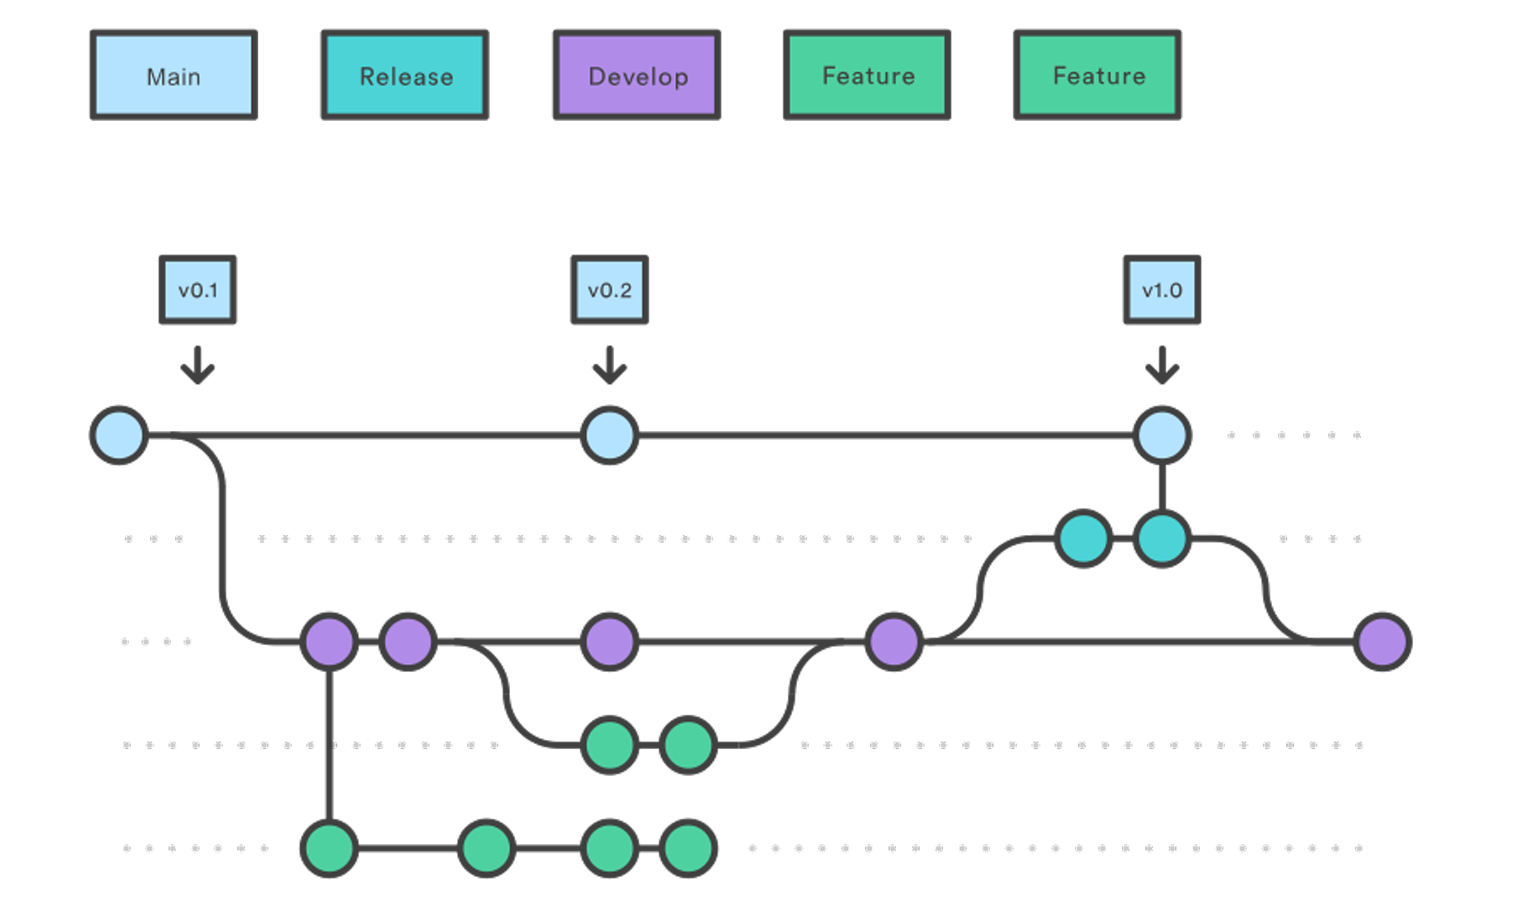
\includegraphics[width=0.9\textwidth]{images/gitWorkflow.png}
    \caption{Git Workflow}
    \label{fig:git-workflow}
\end{figure}

For each new feature or bug fix, we create a feature branch from develop. Once the work is completed and tested, it is merged back into develop through a pull request process. This ensures code review and quality control before any changes are integrated. When a release is ready, develop is merged into main, creating a new stable version of the application.

\section{Product backlog}

The backlog was created before the sprints to plan the milestones and determine the content of each sprint based on project needs \cite{ProductBacklogGuide2024, SchwarzScrum2019}. It includes the following fields:
\begin{itemize}
    \item \textbf{Code:} The unique identifier of the task.
    \item \textbf{Theme:} The subject of a user story.
    \item \textbf{User Story:} A short description of the functionality requested by the client.
    \item \textbf{Priority:} A value indicating the importance of the functionality \cite{MoscowMethodology2021, CleggCaseMethod2004}.
    \begin{itemize}
        \item \textbf{Must:} The feature is essential and must be implemented.
        \item \textbf{Should:} The feature should be implemented if possible.
        \item \textbf{Could:} The feature is optional and may be deprioritized.
        \item \textbf{Won't:} The feature is not a priority at this time.
    \end{itemize}
\end{itemize}

Table \ref{tab:product-backlog} shows the product backlog for our Korpor project:

\begin{longtable}{|c|l|p{8cm}|c|}
    \caption{Korpor Product Backlog\label{tab:product-backlog}} \\
        \hline
        \textbf{Code} & \textbf{Theme} & \textbf{User story} & \textbf{Priority} \\
        \hline
    \endfirsthead
    
    \hline
    \endhead
    
    \hline \multicolumn{4}{|r|}{{Continued on next page}} \\ \hline
    \endfoot
    
    \hline
    \endlastfoot
    
    % Authentication & User Management section
    \multicolumn{4}{|c|}{\cellcolor{primary!15}\textbf{\textcolor{primary}{Authentication \& User Management}}} \\
    \hline
    PB001 & Authentication & As a user, I want to create an account and authenticate securely & Must \\
    \hline
    PB002 & User Management & As a user, I want to manage my profile information & Must \\
    \hline
    PB003 & Authentication & As a user, I want to securely reset my password & Must \\
    \hline
    PB004 & Admin Management & As a Super Admin, I want to manage admin accounts for different real estate companies & Should \\
    
    
    % Super Admin Features section
    \multicolumn{4}{|c|}{\cellcolor{primary!15}\textbf{\textcolor{primary}{Super Admin Features}}} \\
    \hline
    PB005 & Security & As a Super Admin, I want to monitor security and compliance across the platform & Could \\
    \hline
    PB006 & Configuration & As a Super Admin, I want to configure platform-wide features and settings & Could \\
    \hline
    PB007 & Analytics & As a Super Admin, I want to generate and analyze global performance reports & Could \\
    \hline
    PB008 & Moderation & As a Super Admin, I want to moderate content across the platform & Won't \\
    \hline
    PB009 & AI Integration & As a Super Admin, I want to chat with an AI assistant that can securely access database information & Could \\
    \hline
    


    % Admin Features section
    \multicolumn{4}{|c|}{\cellcolor{primary!15}\textbf{\textcolor{primary}{Admin Features}}} \\
    \hline
    PB010 & Listing Management & As an Admin, I want to manage real estate listings in my company & Must \\
    \hline
    PB011 & Agent Management & As an Admin, I want to oversee real estate agents and their permissions & Should \\
    \hline
    PB012 & Transaction Management & As an Admin, I want to track transactions and calculate agent commissions & Should \\
    \hline
    PB013 & Customer Service & As an Admin, I want to address investor inquiries and issues & Could \\
    \hline
    PB014 & Analytics & As an Admin, I want to access a comprehensive agency dashboard & Could \\
    \hline
    PB015 & AI Integration & As an Admin, I want to input property details and receive AI-powered valuation & Should \\
    \hline
    
    % Real Estate Agent Features section
    \multicolumn{4}{|c|}{\cellcolor{primary!15}\textbf{\textcolor{primary}{Real Estate Agent Features}}} \\
    \hline
    PB016 & Listing Management & As an Agent, I want to create and manage property listings & Must \\
    \hline
    PB017 & Investment Management & As an Agent, I want to handle investment and purchase requests & Could \\
    \hline
    PB018 & Data Management & As an Agent, I want to contribute data for AI-driven estimates & Could \\
    \hline
    PB019 & Customer Relations & As an Agent, I want to maintain client relationships and communications & Could \\
    \hline
    PB020 & Finance & As an Agent, I want to view my commissions on sales and rentals & Should \\
    \hline
    
    % Investor Features section
    \multicolumn{4}{|c|}{\cellcolor{primary!15}\textbf{\textcolor{primary}{Investor Features}}} \\
    \hline
    PB021 & Property Discovery & As an Investor, I want to browse available property listings & Must \\
    \hline
    PB022 & Search Functionality & As an Investor, I want to filter properties based on my preferences & Could \\
    \hline
    PB023 & Investment Process & As an Investor, I want to invest in properties through a simple process & Could \\
    \hline
    PB024 & Portfolio Management & As an Investor, I want to track my investment portfolio in real-time & Must \\
    \hline
    PB025 & Payment Processing & As an Investor, I want to make secure payments through various methods & Should \\
    \hline
    PB026 & AI Recommendations & As an Investor, I want to receive personalized property recommendations & Must \\
    \hline
    PB027 & AI Assistance & As an Investor, I want to consult an AI assistant for real estate legal questions & Could \\
    \hline
    PB028 & Financial Prediction & As an Investor, I want to see predictions of potential earnings & Could \\
    \hline
    PB029 & Finance Management & As an Investor, I want to manage my earnings and withdrawals & Could \\
    \hline
    
    % AI & Machine Learning Features section
    \multicolumn{4}{|c|}{\cellcolor{primary!15}\textbf{\textcolor{primary}{AI \& Machine Learning Features}}} \\
    \hline
    PB030 & AI System & As the System, I want to analyze user interactions for personalized recommendations & Must \\
    \hline
    PB031 & AI Prediction & As the System, I want to predict property valuations and rental prices & Should \\
    \hline
    PB032 & AI Forecasting & As the System, I want to forecast potential investment returns & Should \\
    \hline
    PB033 & NLP Integration & As the System, I want to provide real estate legal information via NLP & Could \\
    \hline
    PB034 & Security & As the System, I want to secure AI database access for authorized queries & Could \\
    \hline
    
    % Blockchain & Smart Contract Features section
    \multicolumn{4}{|c|}{\cellcolor{primary!15}\textbf{\textcolor{primary}{Blockchain \& Smart Contract Features}}} \\
    \hline
    PB035 & Blockchain & As the System, I want to create and manage virtual contracts for transactions \cite{WangBlockchainRealEstate2023} & Must \\
    \hline
    PB036 & Blockchain & As an Investor, I want my property investments to be secured via blockchain \cite{McKinseyBlockchainRE2023} & Must \\
    \hline
    PB037 & Blockchain Management & As an Admin, I want to verify and validate blockchain transactions & Should \\
    \hline
    PB038 & Data Integrity & As the System, I want to store transaction records immutably on blockchain & Must \\
    \hline
    PB039 & System Monitoring & As a Super Admin, I want to monitor blockchain health and performance & Should \\
    \hline
    
    % System & Security Features section
    \multicolumn{4}{|c|}{\cellcolor{primary!15}\textbf{\textcolor{primary}{System \& Security Features}}} \\
    \hline
    PB040 & Authentication & As the System, I want to automate authentication and session management & Should \\
    \hline
    PB041 & Notifications & As the System, I want to generate real-time notifications for relevant users & Could \\
    \hline
    PB042 & Data Consistency & As the System, I want to maintain transaction consistency across the platform & Should \\
    \hline
    PB043 & Security & As the System, I want to ensure secure communication between AI and database & Should \\
    \hline
    
    % DevOps & Infrastructure section
    \multicolumn{4}{|c|}{\cellcolor{primary!15}\textbf{\textcolor{primary}{DevOps \& Infrastructure}}} \\
    \hline
    PB044 & CI/CD & As a Developer, I want CI/CD pipelines to build project images on GitHub \cite{ForsgreniDevOpsMetrics2023} & Must \\
    \hline
    PB045 & Deployment & As a Developer, I want to automate image deployment to GCP registry & Must \\
    \hline
    PB046 & Deployment & As a Developer, I want to auto-deploy backend services and database & Must \\
    \hline
    PB047 & Containerization & As a Developer, I want to containerize application components with Docker & Must \\
    \hline
    PB048 & Web Deployment & As a Developer, I want to automatically deploy the web app frontend & Should \\
    \hline
    PB049 & Mobile Deployment & As a Developer, I want to automate mobile app deployments to Play Store & Should \\
    \hline
    PB050 & Versioning & As a Developer, I want to implement versioning for mobile app releases & Should \\
    \hline
    PB051 & Monitoring & As an Admin, I want to monitor system health and performance & Could \\
    \hline
    PB052 & Configuration & As a Super Admin, I want to manage environment configurations & Could \\
        \hline
    
    % Mobile App Specific Features section
    \multicolumn{4}{|c|}{\cellcolor{primary!15}\textbf{\textcolor{primary}{Mobile App Specific Features}}} \\
    \hline
    PB053 & Mobile UI/UX & As an Investor, I want a responsive, intuitive mobile interface \cite{NielsenResponsiveDesign2019} & Should \\
    \hline
    PB054 & Notifications & As an Investor, I want to receive push notifications about my investments & Should \\
    \hline
    PB055 & Offline Access & As an Investor, I want offline access to my basic portfolio information & Should \\
\end{longtable}

\section{Sprint planning}

In order to complete the project within the deadlines set by the internship agreement, planning is an important step in the process \cite{SutherlandScrum2020, RubinEssentialScrum2012}. It was therefore necessary to define the essential steps and estimate the time to be devoted to the completion of the various tasks. To do this, we made a GANTT chart.

In our project management, we opted for the proportional distribution method in order to estimate the costs \cite{CohnAgileEstimating2005, GreningPlanningPoker2002}.
Figure \ref{fig:gantt-chart} shows the Gantt chart that describes the progress of our project:

\vspace{1cm}
\newpage

\begin{figure}[htbp]
    \centering
    % Replace with actual image file once available
    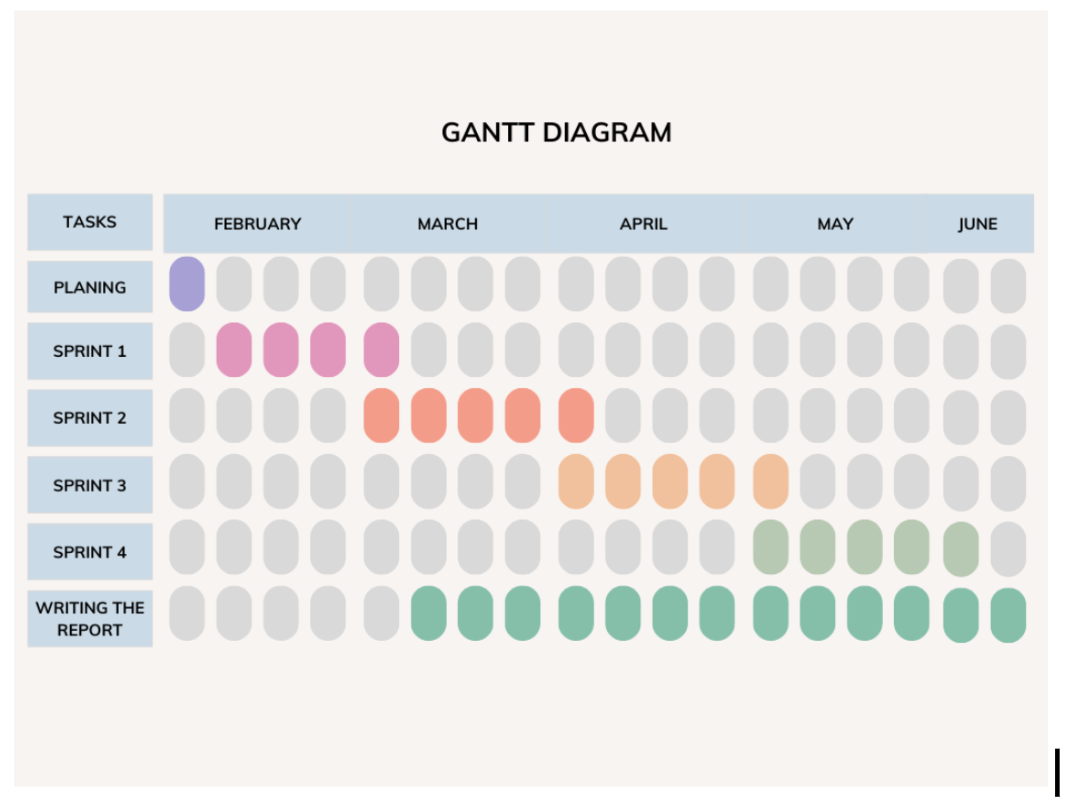
\includegraphics[width=0.7\textwidth]{images/gantt-chart.png}
    \caption{GANTT chart with sprint planning}
    \label{fig:gantt-chart}
\end{figure}

% \vspace{2cm}

\section*{Conclusion}

Our Sprint 0 marked the exciting start of our KORPOR project \cite{ScaledAgileFramework2024, SutherlandScrum2020}. We defined global and specific objectives, developed a solid architecture, and configured an optimal working environment. With a clear vision of the initial product backlog and preliminary planning for upcoming sprints, we are ready to achieve our vision and achieve our goals successfully \cite{SchwarzScrum2019, RubinEssentialScrum2012}.

